% -*- coding: utf-8; -*-

\chapter{Experimentos}
\label{cap:experimentos}

Este capítulo apresenta os resultados dos experimentos das técnicas de compressão aplicadas a um conjunto de provas de tautologias da M$\supset$.

\section{Ambiente Computacional}

Todos os experimentos relatados nesta Seção foram executados em uma máquina com processador Intel Core i3-6100U 2,30GHz, 8GB de memória RAM e com sistema operacional Ubuntu 18.04.1 LTS. O \textit{gerador de fórmulas}\footnote{\label{ftn:impl_ger_huff}\href{https://github.com/flavio-barros/proof-compressions}{https://github.com/flavio-barros/proof-compressions}} descrito na Seção \ref{sec:base_dados} e a \textit{implementação da codificação de Huffman}\footref{ftn:impl_ger_huff}, cujos resultados de compressão são mostrados na Seção \ref{sec:resultados}, foram implementados utilizando a linguagem \textit{Python}.

\section{Provas de Entrada}
\label{sec:base_dados}

Provas com tamanho super-polinomial em relação ao tamanho da conclusão são redundantes, quanto maior a prova, maior a quantidade de redundâncias \cite{GorHae2019}. Em um árvore de prova, essas redundâncias são ramos idênticos que se repetem ao longo da prova no mesmo nível da derivação. Portanto, para a Compressão Horizontal, quanto maior a prova, maior a quantidade de colapsos e consequentemente, maior a taxa de compressão. Como observado no Capítulo \ref{cap:aplicacao_tec}, quando aplicada a provas que permitem poucos colapsos, a CH gera provas maiores que as originais. Logo, o conjunto de provas utilizadas nos experimentos deve ser necessariamente composto por provas grandes, que possuem tamanhos exponenciais em relação ao tamanho da conclusão, para que seja possível mensurar a capacidade de compressão da CH.

Inicialmente, consideramos três famílias de fórmulas para serem utilizadas nos experimentos. A primeira família de fórmulas $\psi_{n}$ definida em \cite{haeusler2015many}, não possui provas normais, para qualquer $n > 0$, com menos de $2^n$ hipóteses descartadas. $\psi_{n}$ é definida com segue:

\begin{definition}{\textbf{Fórmulas Haeusler.}}
Seja $\chi[X, Y] = (((X \supset Y) \supset X) \supset X) \supset Y$. Considere os símbolos proposicionais $C$ e $D_i$, para $i > 0$. A família de fórmulas $\xi_{i}$ é definida recursivamente como segue:
\begin{align*}
\xi_1 &= \chi[D_1, C] \\
\xi_{i+1} &= \chi[D_{i+1}, \xi_i]
\end{align*}
Utilizando $\xi_i$, a família de fórmulas $\psi_n$, para $n > 0$, é definida como segue, para $i \geq 1$: $$\psi_{i+1} = \xi_{i+1} \supset C$$
\end{definition}

A segunda família de fórmulas foi retirada da Biblioteca ILTP\footnote{\href{http://www.iltp.de/}{http://www.iltp.de/}} (\textit{Intuitionistic Logic Theorem Proving (ILTP) Library}) que fornece uma plataforma para testes para provadores de teoremas da lógica proposicional e de primeira ordem intuicionista. Os problemas da biblioteca estão agrupados em 24 domínios, incluindo o SYJ, domínio dos problemas sintáticos intuicionistas \cite{raths2007iltp}. Um dos problemas, o SYJ204, refere-se a uma família de fórmulas $\phi_n$, tendo apenas a implicação como conectivo, que possui somente provas normais de tamanhos exponenciais. $\phi_n$ é definida como segue:

\begin{definition}{\textbf{Fórmulas SYJ204}.}
Sejam $A_i$, com $i \geq 0$, símbolos proposicionais. A família de fórmulas $\omega_i$ é definida recursivamente como segue:
\begin{align*}
\omega_1 &= (A_1 \supset (A_1 \supset A_0)) \\
\omega_{i+1} &= \omega_i \supset (A_{i+1} \supset (A_{i+1} \supset A_i))
\end{align*}
Utilizando $\omega_i$, a família de fórmulas $\phi_n$, para $n > 0$, é definida como segue, para $i \geq 1$: $$\phi_{i+1} = A_{i+1} \supset (\omega_{i+1} \supset A_0)$$
\end{definition}

A terceira família de fórmulas foi retirada de um exemplo de compressão em \cite{GordeevH16}. $Fib_n$ possui provas normais maiores ou iguais que \textit{fibonacci(n)} e é definida como segue:

\begin{definition}{\textbf{Fórmulas Fibonacci}.}
Sejam $A_i$, com $i \geq 3$, símbolos proposicionais. A família de fórmulas $\sigma_i$ é definida recursivamente como segue:
\begin{align*}
\sigma_3 &= (A_{1} \supset (A_{2} \supset A_{3})) \\
\sigma_{i} &= \sigma_{i-1} \supset (A_{i-2} \supset (A_{i-1} \supset A_{n}))
\end{align*}
Utilizando $\sigma_i$, a família de fórmulas $Fib_n$, para $n > 2$, é definida como segue: $$Fib_{n} = (A_{1} \supset A_2) \supset (\sigma_{n} \supset (A_1 \supset A_n))$$
\end{definition}

As provas utilizadas nos experimentos foram geradas utilizando o provador de teoremas \textit{NatDProver}\footnote{\href{https://github.com/Bpalkmim/NatDProver}{https://github.com/Bpalkmim/NatDProver (Implementação original)}}$^{\text{,}}$\footnote{\href{https://github.com/flavio-barros/NatDProver}{https://github.com/flavio-barros/NatDProver (Implementação alterada para aceitar entradas por linha de comando)}}, desenvolvido no TecMF\footnote{\href{http://www.tecmf.inf.puc-rio.br/}{http://www.tecmf.inf.puc-rio.br/}}, que recebe fórmulas da M$\supset$ e devolve um arquivo \textit{.dot} que contém o grafo de prova caso a prova seja gerada com sucesso. O NatDProver ainda está em desenvolvimento, alguns erros e comportamento inesperados podem ocorrer durante a geração das provas.

Executamos o NatDProver para instâncias das três famílias de fórmulas selecionadas para os experimentos. O provador pode apresentar cinco tipos de retorno em cada execução: \textit{sucesso}, geração da prova e do arquivo \textit{.dot} ocorreram com sucesso; \textit{erro geração DOT}, a geração da prova ocorreu com sucesso, mas a geração do arquivo \textit{.dot} apresentou erro; \textit{erro geração prova}, ocorreu um erro na geração da prova; \textit{falha geração prova}, a geração da prova falhou, mas não ocorreram erros durante a execução; \textit{timeout}, o tempo de execução do provador atingiu o limite de tempo definido.

A Tabela \ref{tab:fam_form_exec} mostra o retorno obtido do NatDProver para cada instância das famílias de fórmulas consideradas. Executamos o provador para 20 instâncias de cada família, o limite de tempo de execução para cada instância foi de 30 minutos.

\begin{table} [!ht]
    \caption{Retornos do NatDProver para cada instâncias das famílias de fórmulas}\label{tab:fam_form_exec}
    ~\\[-2mm]
    \begin{tabularx}{\textwidth}{@{\extracolsep{0pt}}C @{\extracolsep{0pt}} P{2.5cm} C C}

        \hline
        \textbf{Família de fórmulas   } & \textbf{Valor de n} & \textbf{Retorno} \\ \hline
        \multirow{2}{*}{$\psi_n$ (fórmulas Haeusler)} & 1 & \textit{erro geração DOT} \\ \cline{2-3} 
         & 2 - 20 & \textit{falha geração prova} \\ \hline
        \multirow{3}{*}{$\phi_n$ (SYJ204)} & 1 & \textit{sucesso} \\ \cline{2-3} 
         & 2 - 4 & \textit{erro geração DOT} \\ \cline{2-3} 
         & 5 - 20 & \textit{falha geração prova} \\ \hline
        \multirow{2}{*}{$Fib_n$ (fórmulas Fibonacci)} & 3 - 15 & \textit{sucesso} \\ \cline{2-3} 
         & 16 - 22 & \textit{timeout} \\ \hline
    \end{tabularx}
\end{table}

Após as execuções, o NatDProver não gerou nenhum arquivo \textit{.dot} com provas das fórmulas Haeusler, um arquivo para as fórmulas SYJ204 e 13 arquivos para as fórmulas Fibonacci. Como o objetivo do experimento é observar as taxas de compressão das provas obtidas por cada técnica a medida que o tamanho das provas aumenta, utilizamos apenas as fórmulas Fibonacci para gerar os resultados mostrados na próxima seção.

\section{Resultados}
\label{sec:resultados}

Nos gráficos seguintes, as provas das fórmulas de $Fib_n$ são mostradas em termos dos tamanhos das fórmulas no lugar dos valores de $n$, a prova da fórmula de $n = 3$ possui a conclusão com tamanho $13$, $n = 4$ possui tamanho $19$, e assim por diante, até $n = 15$ com a conclusão com tamanho $85$.

A Figura \ref{fig:prova_oco_form} mostra o gráfico que relaciona os tamanhos das fórmulas da família $Fib_n$, considerando a quantidade de símbolos proposicionais, e os tamanhos de suas respectivas provas, considerando o tamanho do grafo de prova. Na Figura \ref{fig:prova_siz_form}, os tamanhos das provas são mostrados considerando os tamanhos (em \textit{kilobytes}) dos arquivos DOT que as representa.

\begin{figure}[ht]
  \begin{center}
    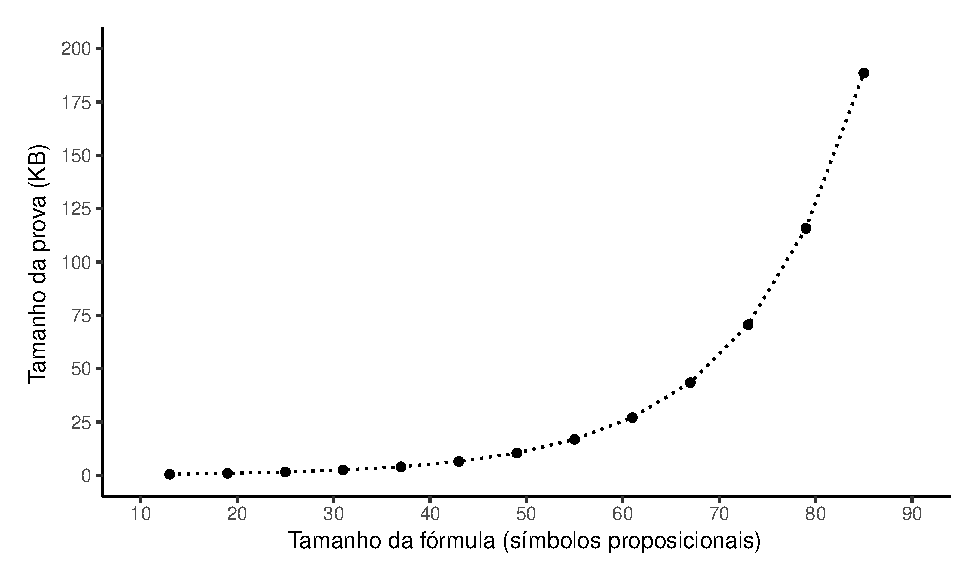
\includegraphics[height=230pt,width=400pt]{images/plot_prova_gra_form.eps}
    \caption{Tamanho das fórmulas e seus respectivos grafos de prova}
    \label{fig:prova_oco_form}
  \end{center}
\end{figure}

\begin{figure}[ht]
  \begin{center}
    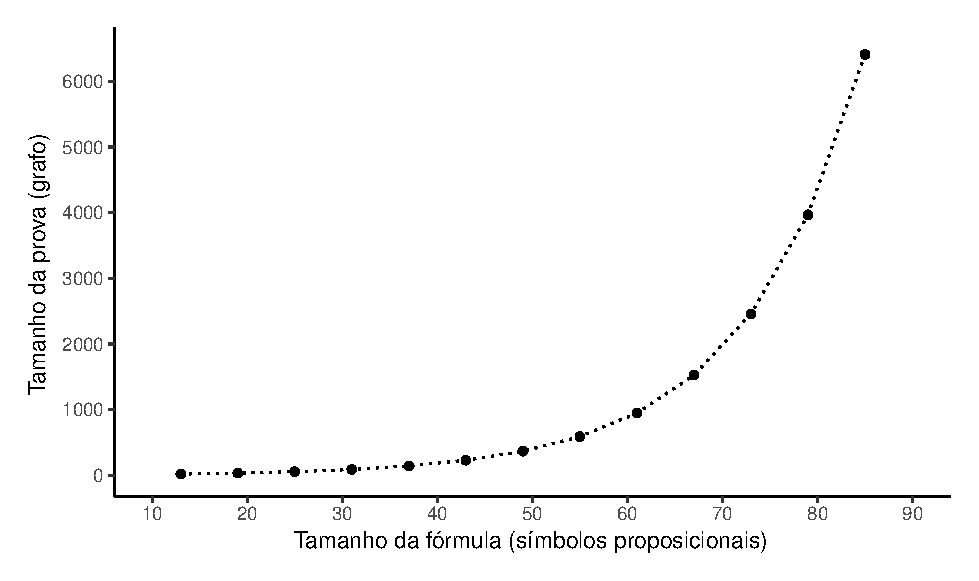
\includegraphics[height=230pt,width=400pt]{images/plot_prova_kb_form.eps}
    \caption{Tamanho das fórmulas e seus respectivos arquivos de prova}
    \label{fig:prova_siz_form}
  \end{center}
\end{figure}

A seguir apresentamos os resultados das aplicações dos algoritmos de compressão às provas das fórmulas de $Fib_n$. Os resultados são mostrados para os algoritmos da codificação de Huffman e da Compressão Horizontal.

A Figura \ref{fig:prova_alg_sizes} mostra os tamanho dos arquivos originais e dos resultantes dos algoritmos de compressão, o eixo dos tamanhos dos arquivos está em escala logarítmica. Como já esperado, a Compressão Horizontal não possui bons resultados para as provas menores, apresentando uma taxa de compressão efetiva apenas a partir da fórmula com tamanho 37 ($n = 7$). A partir da fórmula com tamanho 30 ($n = 8$), a Compressão Horizontal obteve resultados melhores que a codificação de Huffman. A maior prova, da fórmula com tamanho 85 ($n = 15$), possui tamanho original 188,6 KB e foi comprimida para 113 KB pela codificação de Huffman e para 9,36 KB pela Compressão Horizontal.

\begin{figure}[H]
  \begin{center}
    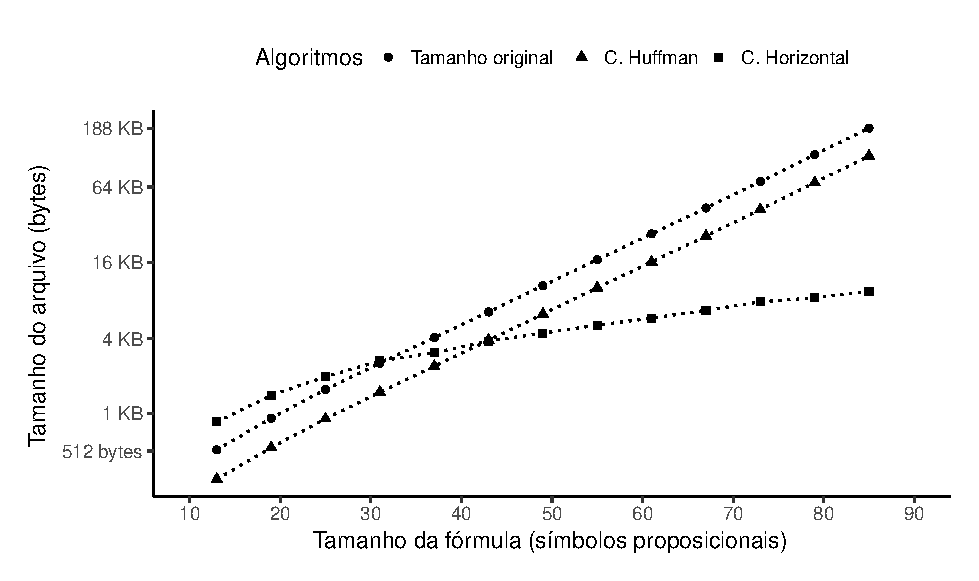
\includegraphics[height=230pt,width=400pt]{images/plot_alg_sizes.eps}
    \caption{Tamanhos dos arquivos de prova após a compressão}
    \label{fig:prova_alg_sizes}
  \end{center}
\end{figure}

A Figura \ref{fig:taxa_comp} mostra as taxas de compressão obtidas para cada fórmula. Para todas as provas, a codificação de Huffman obteve taxa de compressão de aproximadamente 40\%, enquanto que as taxas de compressão da Compressão Horizontal variam bastante de acordo com o tamanho da prova. Para a fórmula de tamanho 13 ($n = 3$), a taxa de compressão obtida foi de -67\% (aumento de 67\% do tamanho do arquivo original) e para a prova da fórmula de tamanho 85 ($n = 15$), a taxa de compressão obtida foi de 95\%.

\begin{figure}[H]
  \begin{center}
    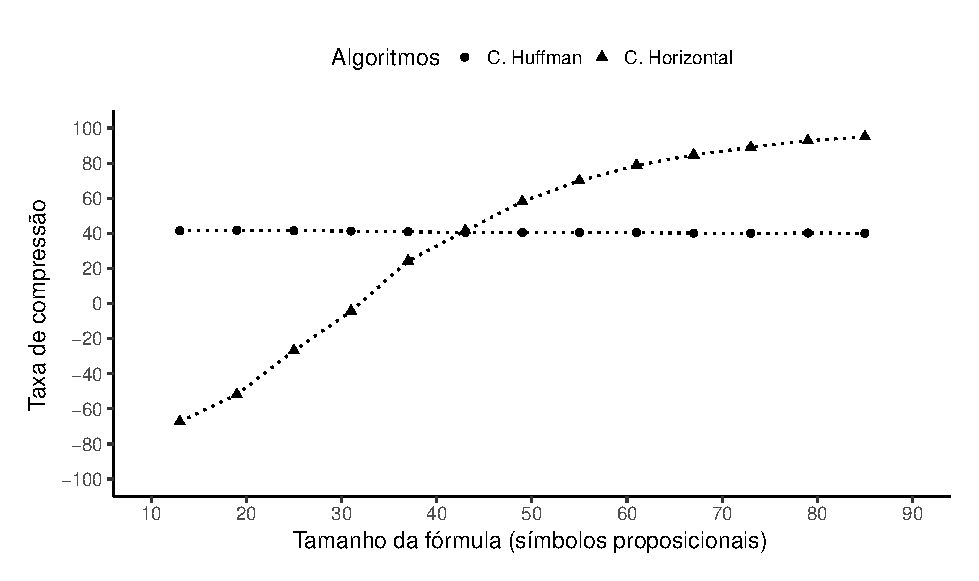
\includegraphics[height=230pt,width=400pt]{images/plot_taxa_comp.eps}
    \caption{Taxa de compressão dos algoritmos}
    \label{fig:taxa_comp}
  \end{center}
\end{figure}

Enquanto que para as taxas de compressão, a Compressão Horizontal obteve resultados mais satisfatórios, para os tempos de execução, a codificação de Huffman apresentou tempos menores para todas as fórmulas. O gráfico da Figura \ref{fig:exec_time} mostra os tempos de execuções dos dois algoritmos para todas as provas, o eixo dos tempos de execução está em escala logarítmica.

\begin{figure}[H]
  \begin{center}
    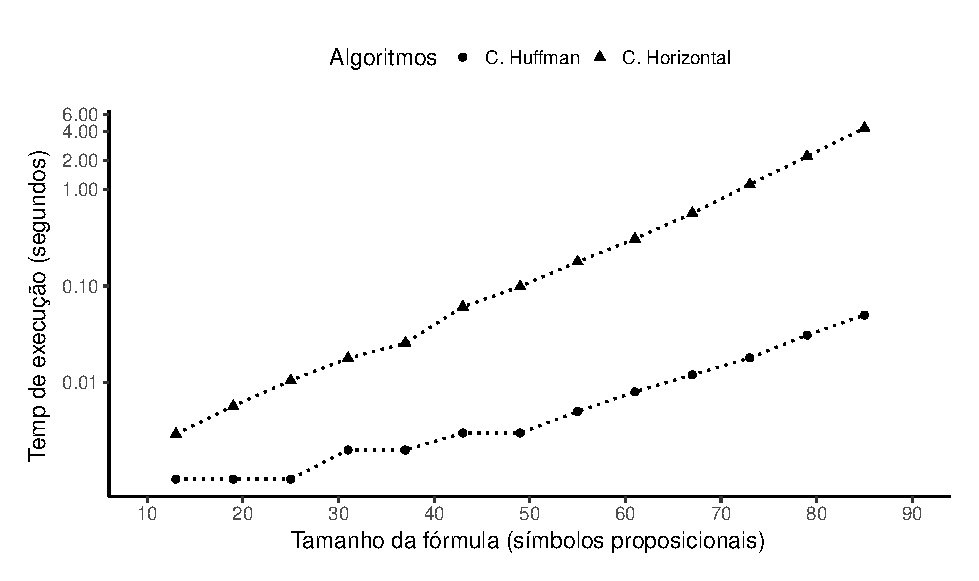
\includegraphics[height=230pt,width=400pt]{images/plot_exec_time.eps}
    \caption{Tempo de execução dos algoritmos de compressão}
    \label{fig:exec_time}
  \end{center}
\end{figure}